\chapter*{Combustió}

\section{El motor de combustió interna}

En un motor de combusti\'o interna (IC) s'introdueix aire i combustible. En els motors d'encesa per espurna, la mescla d'aire i combustible es preparava antigament en el carburador i es condu\"ia al cilindre. Ara es realitza per mitj\`a d'injectors, cosa que permet un estalvi de combustible i un millor aprofitament d'aquest. En els motors d'encesa per compressi\'o (Diesel), la mescla es realitza directament dins del cilindre, on el combustible s'injecta despr\'es d'haver-hi introdu\"it i comprimit l'aire. Cada cilindre del motor t\'e una v\`alvula d'admissi\'o i una d'escapament, que s'obren i tanquen en el moment oport\'u per permetre l'entrada i sortida de gasos. Els motors típics tenen entre 3 i 12 cilindres, i la pot\`encia es pot augmentar afegint m\'es cilindres.

La paret de la cambra de combustió està formada per una camisa de ferro o alumini, i està inserida en un bloc de ferro o acer.

La mescla comprimida a la cambra de combusti\'o es transforma, per efecte de la combusti\'o, en vapor d'aigua (\ch{H2O}), di\`oxid de carboni (\ch{CO2}) i nitrogen (\ch{N2}). El nitrogen, un gas inert contingut a l'aire, no interv\'e en la combusti\'o. El vapor d'aigua produ\"it en la combusti\'o es mant\'e i es comporta com un gas permanent.

Entre els altres productes de la combusti\'o es troben altres gasos com: mon\`oxid de carboni (\ch{CO}), hidrogen (\ch{H2}), metà (\ch{CH4}) i oxigen (\ch{O2}), quan la combusti\'o \`es incompleta. La quantitat d'oxigen que participa en el proc\'es dep\`en directament de l'exc\'es d'aire introdu\"it respecte al necessari per a la combusti\'o.

En conseq\"u\`encia, el fluid de treball est\`a format inicialment per l'aire i el combustible i, despr\'es, pel conjunt de gasos produ\"its durant la combusti\'o. Com \`es evident, la seva composici\'o qu\'imica varia durant el cicle de treball.


\subsection{El motor de quatre temps}

    Un motor de quatre temps és aquell que necessita quatre recorreguts del pistó, dues voltes completes del cigonyal, per completar el seu cicle termodinàmic.

    \newif\ifspark
\tikzset{tangent of circles/.style args={% https://tex.stackexchange.com/a/464143/194703
    at #1 and #2 with radii #3 and #4}{insert path={%
    let \p1=($(#2)-(#1)$),\n1={atan2(\y1,\x1)},\n2={veclen(\y1,\x1)*1pt/1cm},
    \n3={atan2(#4-#3,\n2)}
     in ($(#1)+(\n3+\n1+90:#3)$) coordinate(aux1) -- 
     ($(#2)+(\n3+\n1+90:#4)$) coordinate(aux2)}},
     pics/engine/.style={code={
  \tikzset{engine/.cd,#1}
  \draw[fill=gray!20] (0,0) -- (-0.8,-0.4) coordinate[pos=0.4] (p1)
  coordinate[pos=0.8] (p2) |- (-1,-3)[rounded corners=1mm] |- (-1.2,0) [sharp corners]
  -- (-1.2,0.7) coordinate[pos=0.2] (p3)
  coordinate[pos=0.8] (p4) -- (-0.9,0.85) -- (-0.6,0.7) -- (0,0.4) -- (0.6,0.7)
  -- (0.9,0.85)-- (1.2,0.7) -- (1.2,0)coordinate[pos=0.2] (p6)
  coordinate[pos=0.8] (p5) {[rounded corners=1mm] -- (1,0)}
  [sharp corners] -- (1,-3)
  -| (0.8,-0.4) -- cycle coordinate[pos=0.2] (p8)
  coordinate[pos=0.6] (p7);
  \draw[engine/left exhaust] (p1) to[bend right=18] (p4) -- (p3) to[bend left=18] (p2) -- cycle;
  \draw[engine/right exhaust] (p7) to[bend left=18] (p6) -- (p5) to[bend right=18] (p8) -- cycle;
  \draw[fill=gray!50] (0,-4) circle[radius=5mm];
  \pgfmathsetmacro{\pistonpos}{-4+0.4*sin(\pgfkeysvalueof{/tikz/engine/rod angle})
  +sqrt(1.5*1.5-pow(0.4*cos(\pgfkeysvalueof{/tikz/engine/rod angle}),2))}
  \path (0,-4) + (\pgfkeysvalueof{/tikz/engine/rod angle}:0.4) coordinate (p9)
   (0,\pistonpos) coordinate (p10);
  \draw[fill=gray!15] (p9) circle [radius=2mm] -- (p10) circle [radius=1mm];
  \path[tangent of circles={at p10 and p9 with radii 0.1 and 0.2}]
  (aux1) coordinate (aux3) (aux2) coordinate (aux4); 
  \path[tangent of circles={at p9 and p10 with radii 0.2 and 0.1}];
  \path[fill=gray!15] (aux1) -- (aux2) -- (aux3) -- (aux4);
  \draw  (aux1) -- (aux2)  (aux3) -- (aux4);
  \path[fill=gray!45] (p9) circle [radius=1.2mm];
  \begin{scope}
   \clip (-0.8,\pistonpos)   rectangle ++ (1.6,1);
   \draw[left color=gray!60,right color=gray!50,middle color=gray!10] (-0.8,\pistonpos) 
  rectangle ++ (2,1);
  \end{scope}
  \draw[left color=\pgfkeysvalueof{/tikz/engine/interior color}!80,
  right color=\pgfkeysvalueof{/tikz/engine/interior color}!50,
  middle color=white] 
  (-0.8,\pistonpos+1) --  (-0.8,-0.4)  -- (0,0)--  (0.8,-0.4) |- cycle;
  \draw[thin,fill=gray!30] (-0.42,-0.5) 
   ++ ({90+atan(1/2)}:0.25*\pgfkeysvalueof{/tikz/engine/left valve}) 
   -- ++ ({90+atan(1/2)}:1.9) -- ++ ({atan(1/2)}:0.1)
   -- ++ ({-90+atan(1/2)}:1.9) -- ++({atan(1/2)}:0.3)
   -- ++ ({-90+atan(1/2)}:0.1) -- ++({atan(1/2)+180}:0.7)
   -- ++ ({90+atan(1/2)}:0.1) -- cycle;
  \draw[thin,fill=gray!30] (0.42,-0.5) 
   ++ ({90-atan(1/2)}:0.25*\pgfkeysvalueof{/tikz/engine/right valve}) 
   -- ++ ({90-atan(1/2)}:1.9) -- ++ ({180-atan(1/2)}:0.1)
   -- ++ ({-90-atan(1/2)}:1.9) -- ++({180-atan(1/2)}:0.3)
   -- ++ ({-90-atan(1/2)}:0.1) -- ++({-atan(1/2)}:0.7)
   -- ++ ({90-atan(1/2)}:0.1) -- cycle;
  \draw[left color=gray!60,right color=gray!50,middle color=gray!10]
   (-0.1,-0.2) rectangle (0.1,1);   
  \ifspark
  \begin{scope}
   \clip (-1.8,-0.2) rectangle (1.8,\pistonpos+1.1);
   \path (0,-0.2) node[starburst, inner color=yellow, outer color=red,minimum size=1cm]{};
  \end{scope}
  \fi 
 }},engine/.cd,left valve/.initial=1,right valve/.initial=1,
 left exhaust/.style={fill=gray!50},
 right exhaust/.style={fill=gray!50},
 rod angle/.initial=30,interior color/.initial=white,
 spark/.is if=spark}
 \begin{center}
 \scalebox{0.8}{
\begin{tikzpicture}[] 
 \path (0,0) pic{engine={left valve=0,rod angle=-40,
  left exhaust/.style={fill=gray!10}}}
 (3.2,0) pic{engine={rod angle=-170,interior color=yellow}}
 (6.4,0) pic{engine={rod angle=105,interior color=orange,spark}}
 (9.6,0) pic{engine={rod angle=-80,interior color=red}}
 (12.8,0) pic{engine={right valve=0,rod angle=-170,interior color=purple,
    right exhaust/.style={fill=purple!30}}};
\end{tikzpicture}
 }
\end{center}

\begin{itemize}

\item{Primer pas o admissió}
En aquesta etapa, quan el pistó baixa des del Pnt Mort superior (PMS) al Punt Mort Inferior (PMI), permet que el nou combustible entri per la vàlvula d'injecció. Mentre s'obre aquesta vàlvula, la d'escapament es manté tancada.

\item{Segon pas o compressió}
Al final de l'execució anterior, el gas dins del cilindre es comprimeix per mitjà del moviment ascendent del pistó, de manera que la vàlvula d'injecció es tanca per la pressió.

\item{Tercer pas o explosió/expansió}
Després del temps de compressió, quan el pistó torna a la posició superior, s'obté la pressió màxima dins del cilindre. En el nostre cas, tenim un motor dièsel, per la qual cosa el combustible s'injecta polvoritzat i es crema per mitjà de la pressió i la temperatura dins del cilindre. Aleshores, l'expansió del gas fa que el pistó es mogui de nou cap avall; és en aquest moment quan es crea el treball de tot el procés. El treball d'expansió obtingut és aproximadament cinc vegades el treball de compressió necessari.

\item Quart pas o escapament
En aquest últim pas, el moviment superior del pistó fa que els gasos de combustió surtin a través de la vàlvula d'escapament. Quan el pistó està a la part superior, la vàlvula d'escapament es tanca i la injecció s'obre perquè tot el procés es torni a iniciar.
\end{itemize}

El cigonyal completa dues voltes (720 graus) per cada cicle de quatre temps. Així, el motor de quatre temps necessita dues voltes completes del cigonyal per completar el seu cicle termodinàmic.

Molts dels comportaments del motor es poden descriure mitjan\c{c}ant els conceptes de les lleis dels gasos. Per exemple, segons la llei de Boyle, quan augmenta el volum de la cambra de combusti\'o durant l'aspiraci\'o, la pressi\'o disminueix i permet que l'aire entri al cilindre. Durant la compressi\'o, el gas s'escalfa i augmenta la pressi\'o. L'expansi\'o dels gasos calents, descrita per la llei de Charles, \`es el mecanisme pel qual es captura l'energia de la combusti\'o i es converteix en energia mec\`anica per impulsar el vehicle\cite{bowers_understanding_2014}.

    \subsection{Fases del Cicle Otto ideal}

    Els processos termodinàmics que es donen en el cicle Otto es poden resumir en\cite{morales_caracterizacion_nodate}:
\begin{enumerate}
    \item 0-1 Aspiraci\'o (proc\'es isoc\`oric): 
    La v\'alvula d'admissi\'o s'obre i s'aspira una c\`arrega d'aire i combustible a una pressi\'o te\`oricament igual a l'atmosf\`erica, provocant el descens del pist\'o. La v\'alvula d'escapament roman tancada. L'injector de fuel  genera un aerosol de combustible, en forma d'una fina boira de gotes minúscules, que es barreja amb l'aire aspirat.
    
    \item 1-2 Compressi\'o (proc\'es adiab\`atic):
    No existeix intercanvi de calor entre el gas i les parets del cilindre. La v\'alvula d'admissi\'o i la d'escapament estan tancades i el pist\'o comen\c{c}a a pujar, comprimint la mescla que es vaporitza.
    
    \item 2-3 Combusti\'o (proc\'es isoc\`oric):
    Ambdues v\'alvules romanen tancades. Quan el pist\'o arriba a la part superior del seu recorregut, el gas comprimit s'inflama per l'espurna de la bugia. La combusti\'o de tota la massa gasosa \`es instant\`ania, per la qual cosa el volum no variar\`a i la pressi\'o augmentar\`a r\`apidament. Això és degut a que la reacció genera molts més mols de gas que els inicials, i la temperatura augmenta enormement degut a la reacció química.
    
    \item 3-4 Expansi\'o (proc\'es adiab\`atic): 
    El gas inflamat empeny el pist\'o. Durant l'expansi\'o, no hi ha intercanvi de calor i, en augmentar el volum, la pressi\'o tamb\'e augmenta.
    
    \item 4-1 Escapament (proc\'es isoc\`oric)
    Quan el pist\'o es troba en l'extrem inferior del seu recorregut, la v\'alvula d'admissi\'o roman tancada i s'obre la d'escapament, disminuint r\`apidament la pressi\'o sense variar el volum interior. Despr\'es, mantenint la pressi\'o igual a l'atmosf\`erica, el volum disminueix.
\end{enumerate}
    
    
        \begin{figure}
            \centering
    \begin{tikzpicture}[annotate/.style 2 args={postaction={decorate,decoration={markings,
        mark=at position 0 with {\node[circle,inner sep=1.5pt,draw,fill=white,#1]{};},
        mark=at position 0.5 with {\arrow[>=stealth,line width=1.5pt]{>};
        \node at (0,0.4) {#2};}}}}]
         \draw[stealth-stealth] (0,5) node[below left]{$p$} |- (5,0) node[below left]{$V$};
         \begin{scope}[thick]
          \draw[annotate={label=below right:1,alias=1}{$\dbar Q=0$}] plot[variable=\x,domain=4:1.5] (\x,{5/(\x+3)});
          \draw[annotate={label=below left:2,alias=2}{}] (1.5,5/4.5) -- (1.5,15/4.5);
          \draw[annotate={label=above left:3,alias=3}{$\dbar Q=0$}] plot[variable=\x,domain=1.5:4] (\x,{15/(\x+3)});
          \draw[annotate={label=above right:4,alias=4}{}] (4,15/7) -- (1);  
         \end{scope} 
         \path (2) -- (3) coordinate[pos=0.5] (23) (1) -- (4) coordinate[pos=0.5] (14);
         \draw[stealth-] ([xshift=-2mm]23) -- ++ (-1,0) node[midway,above]{$\Delta Q_h$};
         \draw[-stealth] ([xshift=2mm]14) -- ++ (1,0) node[midway,above]{$\Delta Q_c$};
         \draw[dashed] (1) -- (1|-0,0) node[below] {$V_1$};
         \draw[dashed] (2) -- (2|-0,0) node[below] {$V_2$};
        \end{tikzpicture}
        \caption{La termodinàmica del cicle d'Otto. Els processos d'expansió i compressió són adiabàtics, mentre que els de combustió i escapament són isocòrics.}
    \end{figure}

    \subsection{Cicle Otto Real}

    \begin{enumerate}
        \item 0-1 Aspiraci\'o: 
        La pressi\'o del gas durant l'aspiraci\'o \'es inferior a la pressi\'o atmosf\`erica, per tant, el tancament de la v\'alvula d'admissi\'o es produeix despr\'es que el pist\'o arriba a l'extrem inferior de la seva carrera. Aix\`o prolonga el per\'iode d'admissi\'o i permet l'entrada de la m\`axima quantitat de mescla d'aire i combustible al cilindre.
        
        \item 1-2 Compressi\'o:
        El gas cedeix calor al cilindre, cosa que fa que es refredi i adquireixi menys pressi\'o.
        
        \item 2-3 Combusti\'o:
        La combusti\'o no \`es instant\`ania i el volum de la mescla varia mentre es propaga la inflamaci\'o. Per obtenir un m\`axim treball, \'es essencial triar el moment adequat per a l'encesa. La xispa ha de saltar abans que el pist\'o hagi finalitzat la carrera de compressi\'o, cosa que augmenta considerablement la pressi\'o assolida despr\'es de la combusti\'o i, per tant, el treball guanyat.
        
        \item 3-4 Expansi\'o: 
        L'augment de temperatura dins del cilindre durant la combusti\'o fa que, durant l'expansi\'o, els gasos cedeixin calor al cilindre i es refredin, resultant en una pressi\'o menor.
        
        \item 4-1 Escapament:
        En realitat, l'escapament no es produeix instant\`aniament. Els gasos encara tenen una pressi\'o superior a l'atmosf\`erica en aquest per\'iode. Per aix\`o, la v\'alvula d'escapament s'obre abans que el pist\'o arribi a l'extrem inferior del seu recorregut, permetent que la pressi\'o del gas disminueixi a mesura que el pist\'o acaba la seva carrera descendent. Quan el pist\'o realitza la seva carrera ascendent, troba davant seu gasos ja gaireb\'e totalment expandits. A m\'es, la v\'alvula d'admissi\'o s'obre abans que el pist\'o arribi a l'extrem superior del seu recorregut, generant una certa depressi\'o en el cilindre que afavoreix una aspiraci\'o m\'es en\`ergica.
    \end{enumerate}



\subsection{Cicle Diesel}

El motor Diesel \`es un motor de combusti\'o interna basat en el cicle Otto, per\`o amb la difer\`encia que el combustible s'injecta despr\'es de la compressi\'o de l'aire. 

Durant l'aspiraci\'o, entra nom\'es aire en el cilindre. En la compressi\'o, l'aire s'escalfa i, quan el pist\'o arriba al punt mort superior, s'injecta el di\`esel. Un motor diesel presenta uns factors de compressió molt més elevats que un motor Otto, i per tant, la temperatura de l'aire comprimit és molt més alta. Això permet que el dièsel s'encengui per la pressió i la temperatura de l'aire comprimit, sense necessitat d'una espurna. Finalment, l'escapament funciona de manera similar al motor d'encesa per espurna. 

Aquest motor permet una major efici\`encia t\'ermica i t\'e avantatges econ\`omics en diverses aplicacions. Tot i aix\`o, presenta dificultats t\`ecniques en sistemes d'injecci\'o i combusti\'o. Per garantir una combusti\'o neta i eficient, el proc\'es es realitza en mil\`lisegons. Els motors Diesel usen ratios combustible/aire molt més baixos, amb la qual cosa la combustió és més completa.





    \section{Reaccions de combustió}

    Per definici\'o, una reacci\'o de combusti\'o \`es qualsevol reacci\'o entre un material i un oxidant [t\'ipicament \ch{O2 (g)}] que allibera energia en forma de calor. Les reaccions qu\'imiques alteren els tipus d'enlla\c{c}os i les posicions relatives dels \`atoms dins de les mol\'ecules. Els materials inicials s'anomenen reactius, i els materials finals despr\'es de la reordenaci\'o s'anomenen productes. En una reacci\'o de combusti\'o, el material inicial no oxidant s'anomena combustible i pot ser una varietat de compostos qu\'imics\cite{bowers_understanding_2014}.

Normalment, la combusti\'o es presenta en qu\'imica general i org\`anica com la reacci\'o dels combustibles hidrocarbonats amb l'oxigen per produir di\`oxid de carboni i aigua:
\begin{equation}
\ch{CH4 + 2O2 -> CO2 + 2H2O}
\end{equation}

No obstant aix\`o, els combustibles org\`anics contenen m\'es elements que nom\'es carboni i hidrogen, i produeixen altres gasos a banda del di\`oxid de carboni i l'aigua. Els motors de combusti\'o interna tamb\'e generen combustibles hidrocarbonats no cremats i els anomenats NOx t\'ermics, gasos amb la f\'ormula \ch{NO_x} que es formen quan el nitrogen atmosf\`eric es torna molt calent i reacciona amb l'oxigen atmosf\`eric. Aquests gasos contribueixen a les emissions dels motors i es redueixen mitjan\c{c}ant tecnologies d'emissions que es tractaran més endavant.


\subsection{Destil·lació del petroli}

La majoria de motors de combustió interna de gasolina i dièsel estan dissenyats per utilitzar fraccions específiques d'hidrocarburs obtingudes del petroli cru. El petroli és una barreja complexa de compostos orgànics provinents de la descomposició de microorganismes marins enterrats. Només els components més lleugers i volàtils són adequats com a combustible per a vehicles\cite{bowers_understanding_2014}.

Aquests components se separen del petroli mitjançant destil·lació, un procés on el líquid s'escalfa fins a bullir, i els vapors es refreden i es condensen en un recipient. En la destil·lació industrial, això es fa en una torre de destil·lació, un cilindre metàl·lic on els diferents components del petroli es condensen a diferents alçades segons el seu punt d'ebullició. Els compostos més lleugers surten per la part superior com a vapor, mentre que els més pesats es condensen més avall (Figura \ref{fig:torredestillacio}).

\begin{figure}
    \centering
    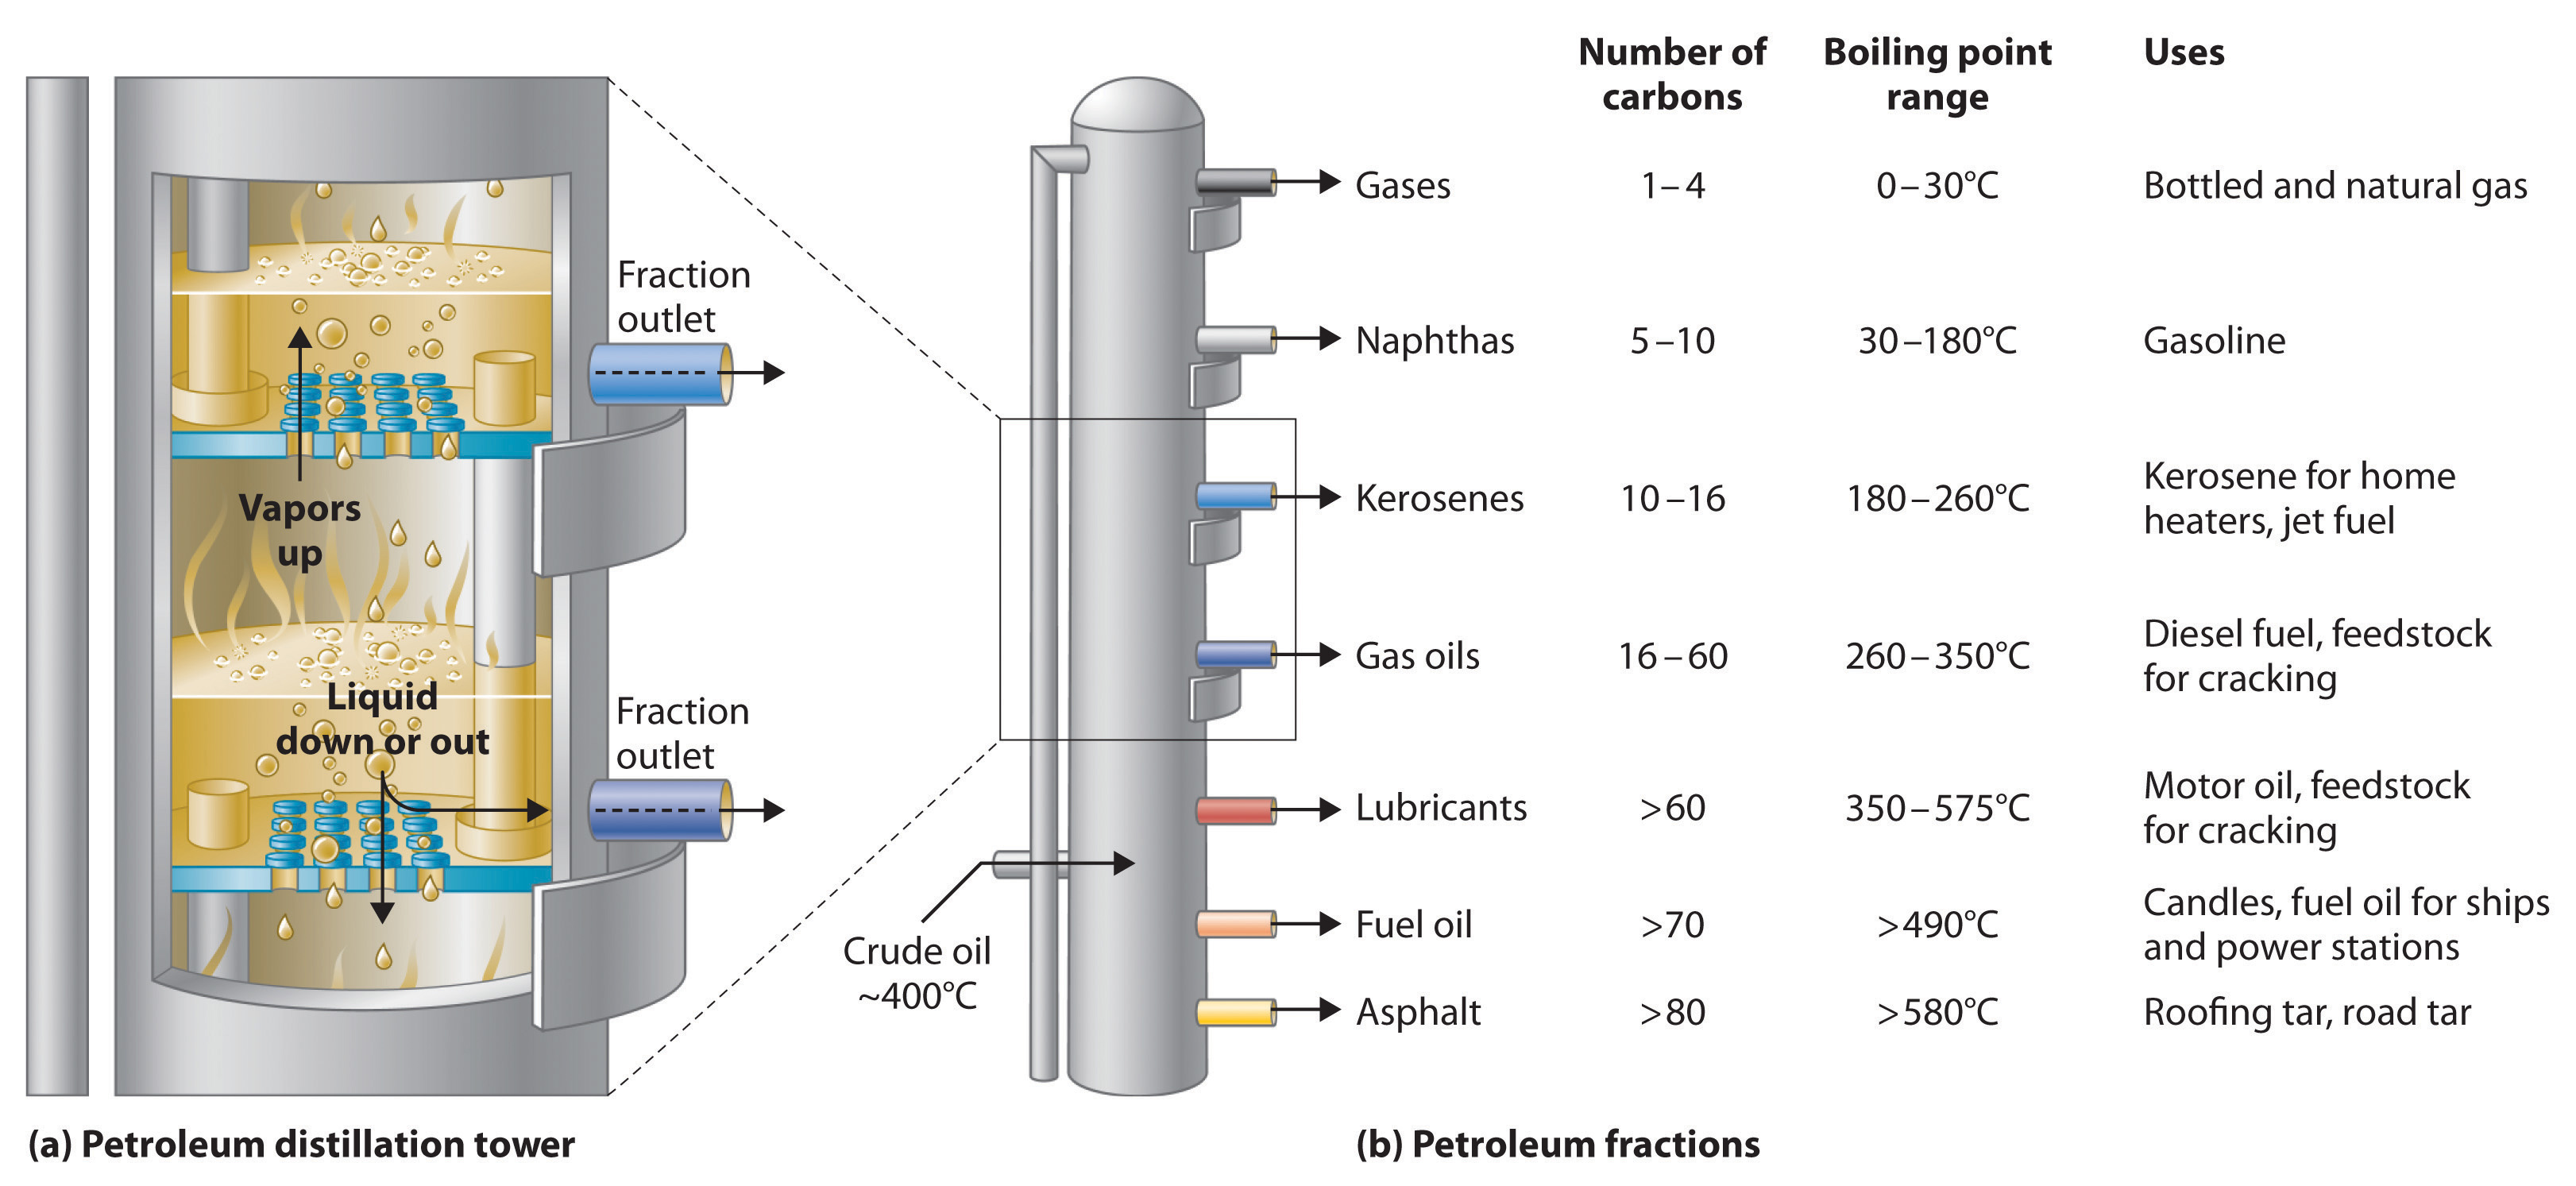
\includegraphics[width=0.8\textwidth]{TorreDestillacio.jpg}
    \caption{Destil·lació fraccionada del petroli\cite{noauthor_38_2015}.}
    \label{fig:torredestillacio}
\end{figure}


El dièsel es destil·la entre 200°C i 350°C i conté hidrocarburs amb entre 8 i 21 àtoms de carboni. La gasolina, més volàtil, conté alcans lieals (parafines), alcans cíclics (naftalens) i alquens (olefines) de 4 a 12 carbonis i es destil·la a temperatures més baixes, pel fet de ser més volàtil. Tant la gasolina com el dièsel inclouen additius químics per millorar la seva estabilitat i resistència a la compressió. Aquests additius solen ser substàncies orgàniques contenir nitrogen, fòsfor i oxigen, i també compostos aromàtics (anells de carboni amb enllaços híbrids).

Per simplificar, l'anàlisi de la combustió es centrarà en la gasolina i un dels seus principals components, l'octà, tot i que el mateix principi s'aplica a altres combustibles.

\subsection{L'índex d'octà}


    Què significa el número d'octà de la benzina o per què alguns cotxes necessiten gasolina premium? El número d'octà mesura la resistència del combustible a la ignició espontània quan es comprimeix.

    L'octà, o n-octà, és un hidrocarbur de la família dels alquans amb fórmula molecular \ch{C8H18}. És un líquid incolor, inodor i inflamable. És un component important de la gasolina, ja que té una estructura lineal que li permet tenir una alta resistència a la detonació. Això fa que sigui un combustible ideal per a motors d'alta compressió.


En un motor de combustió interna, el combustible ha de cremar quan s'encén la bugia. Si la compressió fa que es detoni abans d'horaes poden danyar components com vàlvules i pistons. Això es coneix com a picat de biela o preignició.

El número d'octà es determina en un laboratori, cremant el combustible en un motor amb ràtio de compressió variable fins que es detecta el picat. A partir d'això, es compara amb una barreja de \href{https://www.ebi.ac.uk/chebi/searchId.do?printerFriendlyView=true&chebiId=62805&structureView=applet}{isooctà} i heptà amb la mateixa resistència a la detonació. El número d'octà indica el percentatge d'isooctà en aquesta barreja equivalent. Per exemple, un combustible amb un número d'octà de 90 té la mateixa resistència a la preignició que una barreja del 90\% d'isooctà i 10\% d'heptà (veure Taula \ref{tab:octa}).

És important saber que aquest número no indica la quantitat real d'octà en la benzina. Hi ha altres compostos amb més resistència a la detonació que poden donar valors superiors a 100. En resum, com més alta sigui la ràtio de compressió del motor, més alt ha de ser el número d'octà per evitar problemes de preignició.

\begin{table}[h]
    \centering
    \renewcommand{\arraystretch}{1.5}
    \begin{tabular}{|p{1cm}|c|c||p{1cm}|c|c|}
        \toprule
        \textbf{Nom} & \textbf{Fórmula } & \textbf{Índex} & \textbf{Nom} & \textbf{Fórmula } & \textbf{Índex} \\
        \midrule
        n-heptà & \ch{CH3-(CH2)5-CH3} & 0 &
        o-xilè & \chemfig{[:-30]**6(--(-CH3)-(-CH3)--(-[,,,,,draw=none])-)} & 107 \\
        n-hexà & \ch{CH3-(CH2)4-CH3} & 25 &
        etanol & \ch{CH3CH2OH} & 108 \\
        n-pentà & \ch{CH3-(CH2)3-CH3} & 62 &
        t-butil alcohol & \ch{(CH3)3COH} & 113 \\
        isooctà & \ch{(CH3)3CCH2CH(CH3)2} & 100 &
        p-xilè & \chemfig{[:-30]**6((-CH3)---(-CH3)---)} & 116 \\
        benzè & \chemfig{[:-30]**6(------)} & 106 &
        metil terc-butil èter & \ch{H3COC(CH3)3} & 116 \\
        metanol & \ch{CH3OH} & 107 &
        toluè & \chemfig{[:-60]*6(-=-=(-CH3)-=)} & 118 \\
        \bottomrule
    \end{tabular}
    \caption{Taula de compostos amb les seves fórmules condensades i índex d'octà (Adaptada de \cite{noauthor_38_2015}). }
    \label{tab:octa}
\end{table}

Molts compostos actuals tenen un índex d'octà superior a 100, cosa que els fa millors combustibles que l'isooctà pur. A més, s'han desenvolupat agents anticolp, també anomenats potenciadors d'octà. Durant molts anys, un dels més utilitzats va ser el tetraetilplom \ch{(C2H5)4Pb}, que a una concentració d'aproximadament 3 g/gal augmentava l'índex d'octà en 10-15 punts. No obstant això, des de 1975, els compostos de plom han estat eliminats com a additius de la gasolina a causa de la seva elevada toxicitat.

Per substituir-los, es van desenvolupar altres potenciadors com el metil terc-butil èter (MTBE), que té un índex d'octà elevat i causa poca corrosió al motor i al sistema de combustible. Tanmateix, les fuites de gasolina amb MTBE des de dipòsits subterranis han contaminat aigües subterrànies en algunes zones, fet que ha portat a restriccions o prohibicions del seu ús. Com a alternativa, s'està promovent l'ús d'etanol, que es pot obtenir de fonts renovables com el blat de moro, la canya de sucre i, en el futur, tiges de blat de moro i gramínies.

%\section{Convertidors catalítics}

\newpage
\section{Exercicis}
\begin{exr}
Determina la reacció de combustió de l'octà en presència d'aire.
\end{exr}
\lct{
    La base de càlcul és \qty{1}{\mole} de \ch{C8H18}. Plantegem la reacció de combustió de \qty{1}{\mole} amb $A$ moles d'aire:

    \begin{equation}
        \ch{C8H18} + a(0.21 \ch{O2} + 0.79 \ch{N2}) \ch{-> b CO2 + c H2O + d N2}
    \end{equation}
    
    Els coeficients estequiomètrics $A$, $b$, $c$, $d$ es calculen mitjançant el balanç de les espècies atòmiques C, H, O i N:
    
    \begin{itemize}
        \item Balanç de C: \quad $8 = b$ \quad $\Rightarrow$ \quad $b = \qty{8}{\mole} \ch{CO2}/\qty{1}{\mole} \ch{C8H18}$
        \item Balanç de H: \quad $18 = 2c$ \quad $\Rightarrow$ \quad $c = \qty{9}{\mole} \ch{H2O}/\qty{1}{\mole} \ch{C8H18}$
        \item Balanç de \ch{O2}: \quad $0.21A = b + \frac{c}{2}$ \quad $\Rightarrow$ \quad $A = \qty{59.52}{\mole} \text{aire}/\qty{1}{\mole} \ch{C8H18}$
        \item Balanç de \ch{N2}: \quad $0.79A = d$ \quad $\Rightarrow$ \quad $d = \qty{47.02}{\mole} \ch{N2}/\qty{1}{\mole} \ch{C8H18}$
    \end{itemize}
    
    Així, la reacció teòrica de combustió és:
    
    \begin{equation}
        \ch{C8H18 + 59.52( 0.21 O2 + 0.79 N2 ) -> 8 CO2 + 9 H2O + 47.02 N2}
    \end{equation}
    
    Un mètode alternatiu és plantejar la reacció de combustió en funció només de l'oxigen:
    
    \begin{equation}
        \ch{C8H18} + a \left( \ch{O2} + \frac{79}{21} \ch{N2}\right) \ch{-> b CO2 + c H2O + d N2}
    \end{equation}
    
    Els balanços es fan com segueix:
    
    \begin{itemize}
        \item Balanç de C: \quad $8 = b$ \quad $\Rightarrow$ \quad $b = \qty{8}{\mole} \ch{CO2}/\qty{1}{\mole} \ch{C8H18}$
        \item Balanç de H: \quad $18 = 2c$ \quad $\Rightarrow$ \quad $c = \qty{9}{\mole} \ch{H2O}/\qty{1}{\mole} \ch{C8H18}$
        \item Balanç de \ch{O2}: \quad $a = b + \frac{c}{2}$ \quad $\Rightarrow$ \quad $a = \qty{12.5}{\mole} \ch{O2}/\qty{1}{\mole} \ch{C8H18}$
        \item Balanç de \ch{N2}: \quad $\frac{79}{21}a = d$ \quad $\Rightarrow$ \quad $d = \qty{47.02}{\mole} \ch{N2}/\qty{1}{\mole} \ch{C8H18}$
    \end{itemize}
}
\begin{exr}{Combustió del benzè}
    Si 8,20 g de \ch{C6H6} (benzè) es combinen amb oxigen en una reacció de combustió, quants grams de \ch{H2O} es produiran?
\end{exr}
\lct{
    Equació química equilibrada:
    \[
    \ch{2 C6H6 + 15 O2 -> 12 CO2 + 6 H2O}
    \]
 
    \begin{align*}
    \text{Massa molar de } \ch{C6H6} &= 6(12,01) + 6(1,008) = 78,11 \, \text{g/mol} \\
    \text{Massa molar de } \ch{H2O} &= 2(1,008) + 16,00 = 18,016 \, \text{g/mol}
    \end{align*}
 
          
        \[
        8,20 \cancel{\text{ g } \ch{C6H6}} 
        \times \frac{1 \text{ mol } \ch{C6H6}}{\cancel{78,11 \text{ g } \ch{C6H6}}}
        \times \frac{6 \text{ mols } \ch{H2O}}{2 \cancel{\text{ mols } \ch{C6H6}}}
        \times \frac{18,016 \text{ g } \ch{H2O}}{1 \cancel{\text{ mol } \ch{H2O}}} = 5,68 \text{ g } \ch{H2O}
        \]
}

\begin{exr}{Fòrmula empírica d'un compost petroquímic}
    Després de la combustió en excés d'oxigen, \qty{12,501}{\gram} d'un compost petroquímic van produir 38,196 g de diòxid de carboni i \qty{18,752}{g} d'aigua. Una anàlisi prèvia va determinar que el compost no conté oxigen. Estableix la seva fórmula empírica.
\end{exr}
\lct{Sabem que el compost només conté carboni i hidrogen. L'objectiu és determinar les masses d'aquests elements i trobar la seva relació molar.

Cada mol de \ch{CO2} conté 1 mol de carboni, per tant, utilitzem un factor de conversió:

\[
\text{Massa molar de } \ch{CO2} = 12,01 + 2(16,00) = 44,01 \text{ g/mol}
\]

\[
38,196 \cancel{\text{ g } \ch{CO2} }
\times \frac{1 \cancel{\text{ mol } \ch{CO2}}}{44,01\cancel{ \text{ g } \ch{CO2}}}
\times \frac{1 \cancel{\text{ mol } C}}{1 \cancel{\text{ mol } \ch{CO2}}}
\times \frac{12,01 \text{ g } C}{1 \cancel{\text{ mol } C}}=10,426 \text{ g de } C
\]

Cada mol de \ch{H2O} conté 2 mols d'hidrogen:

\[
\text{Massa molar de } \ch{H2O} = 2(1,008) + 16,00 = 18,016 \text{ g/mol}
\]


\[
18,752 \cancel{\text{ g } \ch{H2O}} 
\times \frac{1\cancel{\text{ mol } \ch{H2O}}}{18,016\cancel{ \text{ g } \ch{H2O}}}
\times \frac{2 \cancel{\text{ mols } H}}{1 \cancel{\text{ mol } \ch{H2O}}}
\times \frac{1,008 \text{ g } H}{1 \cancel{\text{ mol } H}}
=2,100 \text{ g de } H
\]


\[
\text{Massa total calculada} = 10,426 \text{ g C} + 2,100 \text{ g H} = 12,526 \text{ g}
\]
Podem comprovar que el pes de \ch{C} i \ch{H} en els productes iguala el pes dels mateixos elements en els reactius. Com que el valor inicial és de 12,501 g, la diferència es deu a errors d'arrodoniment.

Ara ens interessa veure en quina proporció estan els mols de \ch{C} i \ch{H} en el compost inicial:
\[
\frac{10,426 \text{ g C}}{12,01 \text{ g/mol}} = 0,868 \text{ mols C}
\]
\[
\frac{2,100 \text{ g H}}{1,008 \text{ g/mol}} = 2,083 \text{ mols H}
\]

a partir d'aquests valors podem calcular la fórmula empírica, dividint per qualsevol dels dos i aleshores fent que els valors obtinguts siguin nombres enters: 

\[
\frac{0,868}{0,868} = 1
\]
\[
\frac{2,083}{0,868} = 2,4
\]

Per obtenir nombres enters, multipliquem per 5, i obtenim la fórmula empírica del compost: \ch{C5H12} (pentà). No sabem en quina forma es presentarà, però, el pentà de totes les mostrades a la taula:

\scriptsize
\begin{longtable}{ccc}
    \toprule
    \emph{n}-pentà& \emph{iso}-pentà& \emph{neo}-pentà\\
    \midrule
\definesubmol\xx{C(-[::+90]H)(-[::-90]H)}
\chemfig{H-!\xx-!\xx-!\xx-!\xx-!\xx-H}&
\chemfig{[7]H_3C-CH(-[6]CH_3)-[1]CH_2-CH_3}&
\chemfig{CH_3-C(-[2]CH_3)(-[6]CH_3)-CH_3} 
\\
\bottomrule
\end{longtable}
\normalsize
}

\begin{exr}
    Durant l'anàlisi per combustió d'un compost desconegut que conté només carboni, hidrogen i nitrogen, es van mesurar 12,923 g de diòxid de carboni (\ch{CO2}) i 6,608 g d'aigua (\ch{H2O}).  
    El tractament del nitrogen amb gas \ch{H2} va donar com a resultat 2,501 g d'amoníac (\ch{NH3}).  
    La combustió completa de 11,014 g del compost va necessitar 10,573 g d'oxigen (\ch{O2}).  Quina és la fórmula empírica del compost?
    \end{exr}
\lct{

Càlcul del nombre de mols de carboni
\[
12,923 \text{ g } \ch{CO2} 
\times \frac{1 \text{ mol } \ch{CO2}}{44,011 \text{ g } \ch{CO2}}
\times \frac{1 \text{ mol } C}{1 \text{ mol } \ch{CO2}}
\]

\[
= \frac{12,923}{44,011} = 0,29363 \text{ mols de } C
\]

Càlcul del nombre de mols d'hidrogen
\[
6,608 \text{ g } \ch{H2O} 
\times \frac{1 \text{ mol } \ch{H2O}}{18,02 \text{ g } \ch{H2O}}
\times \frac{2 \text{ mols } H}{1 \text{ mol } \ch{H2O}}
\]

\[
= \frac{6,608 \times 2}{18,02} = 0,7334 \text{ mols de } H
\]

Càlcul del nombre de mols de nitrogen:
\[
2,501 \text{ g } \ch{NH3} 
\times \frac{1 \text{ mol } \ch{NH3}}{17,04 \text{ g } \ch{NH3}}
\times \frac{1 \text{ mol } N}{1 \text{ mol } \ch{NH3}}
\]

\[
= \frac{2,501}{17,04} = 0,1468 \text{ mols de } N
\]


Dividim tots els valors entre el menor nombre de mols (0,1468):

\[
\frac{0,29363}{0,1468} = 2 \quad \text{(mol C)}
\]

\[
\frac{0,7334}{0,1468} = 5 \quad \text{(mol H)}
\]

\[
\frac{0,1468}{0,1468} = 1 \quad \text{(mol N)}
\]

La fórmula empírica del compost és \ch{C2H5N}.

}


\begin{exr}

Calcula l'increment d'energia i d'entalpia en fondre 1 mol de gel. Els volums molars del gel i l'aigua són 0.0196 L/mol i 0.0180 L/mol, respectivament. La calor de fusió de l'aigua és $\Delta H_f = 6.01$ kJ/mol.

\end{exr}

\lct{

Per fondre 1 mol de gel (H$_2$O sòlid) a 0°C i convertir-lo en aigua líquida a 0°C, necessitem conèixer la calor de fusió de l'aigua. La calor de fusió de l'aigua és $\Delta H_f = 6.01$ kJ/mol.

L'increment d'entalpia ($\Delta H$) en fondre 1 mol de gel és simplement la calor de fusió:
\[
\Delta H = \Delta H_f = 6.01 \text{ kJ/mol}
\]

Els volums molars del gel i l'aigua són 0.0196 L/mol i 0.0180 L/mol, respectivament. L'increment d'energia interna ($\Delta U$) es pot calcular utilitzant la relació entre entalpia i energia interna:
\[
\Delta H = \Delta U + P\Delta V
\]
On $P$ és la pressió i $\Delta V$ és el canvi de volum.

El canvi de volum $\Delta V$ es pot calcular com:
\[
\Delta V = V_{\text{líquid}} - V_{\text{sòlid}} = 0.0180 \text{ L/mol} - 0.0196 \text{ L/mol} = -0.0016 \text{ L/mol}
\]

Convertint el canvi de volum a metres cúbics:
\[
\Delta V = -0.0016 \text{ L/mol} \times \frac{1 \text{ m}^3}{1000 \text{ L}} = -1.6 \times 10^{-6} \text{ m}^3/\text{mol}
\]

Assumint que la pressió és 1 atm (101.3 kPa):
\[
P\Delta V = 101.3 \text{ kPa} \times (-1.6 \times 10^{-6} \text{ m}^3/\text{mol}) = -0.000162 \text{ kJ/mol}
\]

Així doncs, l'increment d'energia interna és:
\[
\Delta U = \Delta H - P\Delta V = 6.01 \text{ kJ/mol} - (-0.000162 \text{ kJ/mol}) = 6.010162 \text{ kJ/mol}
\]

Per tant, l'increment d'energia interna en fondre 1 mol de gel és aproximadament 6.01 kJ/mol, i l'increment d'entalpia és 6.01 kJ/mol.
}
\begin{exr}{Energia interna de la combustió del grafit}
Càlcul de $\Delta U$ per a la combustió del grafit a \ch{CO} (gas) en condicions estàndard (\qty{298}{\kelvin} i \qty{1}{\atm}), si l'entalpia de combustió del grafit a \ch{CO} ($\Delta H$): \qty{-110.5}{\kilo\joule\per\mole}. El grafit té un volum molar de \qty{0.0053}{\litre\per\mole}.
\end{exr}

\lct{
La reacció de combustió del grafit a \ch{CO} (gas) es pot escriure com:
\[
\ch{C (grafit)} + \frac{1}{2}\ch{O2} \rightarrow \ch{CO (gas)}
\]

Per calcular el canvi d'energia interna ($\Delta U$) per a aquesta reacció, utilitzarem la relació entre $\Delta U$ i $\Delta H$ (entalpia de reacció):
\[
\Delta U = \Delta H - \Delta(PV)= \Delta H - \Delta n_g RT
\]
on:
\begin{itemize}
    \item $\Delta H$ és l'entalpia de combustió del grafit a \ch{CO}.
    \item $\Delta n_g$ és el canvi en el nombre de mols de gasos.
    \item $R$ és la constant dels gasos ideals (\qty{8.314}{\joule\per\mole\per\kelvin}).
    \item $T$ és la temperatura en Kelvin.
\end{itemize}

Per a la reacció de combustió del grafit a \ch{CO}:
\[
\Delta n_g = n_{\text{productes}} - n_{\text{reactius}} = 1 - \frac{1}{2} = \frac{1}{2}
\]
Un mol de gas a condicions estàndard ocupa un volum de \qty{22.4}{\litre}. Per tant, el canvi de 11.2 litres de gas a \qty{298}{\kelvin} fa que la desaparicció del grafit (\qty{0.0053}{\litre\per\mole}) sigui menyspreable.

Així doncs, $\Delta U$ es calcula com:
\[
\Delta U = \Delta H - \frac{1}{2} RT
\]

L'entalpia de combustió del grafit a \ch{CO} ($\Delta H$) és aproximadament \qty{-110.5}{\kilo\joule\per\mole}. Agafant la temperatura de \qty{298}{\kelvin}:
\begin{align*}
\Delta U &= \qty{-110.5}{\kilo\joule\per\mole} - \frac{1}{2} \cdot \qty{8.314}{\joule\per\mole\per\kelvin} \cdot \qty{298}{\kelvin} \times \qty{e-3}{\kilo\joule\per\joule} \\
&= \qty{-110.5}{\kilo\joule\per\mole} - \qty{1.239}{\kilo\joule\per\mole} \\
&= \qty{-111.739}{\kilo\joule\per\mole}
\end{align*}
}

\begin{exr}{Calor normal de reacció}
Calcula la calor normal de la reacció 
\ch{Fe2O3_{(s)}  + 3 H2_{(g)} <-> 2 Fe_{(s)} + 3 H2O_{(aq)}}
\end{exr}
